\documentclass{article}
\usepackage[spanish]{babel}
\usepackage[utf8]{inputenc}
\usepackage[T1]{fontenc}
\usepackage{blindtext}
\usepackage{geometry}
\usepackage{fancyhdr}
\usepackage{graphicx}
\usepackage[table]{xcolor}
\usepackage[indent=0pt]{parskip}
\usepackage{hyperref}
\usepackage{lastpage}
\usepackage{longtable}
\usepackage{multirow, array} % para las tablas
\usepackage{float} % para usar [H]
\usepackage{xcolor}
\usepackage{xurl}
\usepackage{vmargin}
\usepackage{lscape}

\setpapersize{A4}

\pagestyle{fancy}

\fancyhf{}

\rfoot{\thepage}

\lhead{
\begin{picture}(0,0) \put(0,0){
\includegraphics[width=\textwidth]{./images/encabezado.png}} 
\end{picture}}

\renewcommand{\headrulewidth}{0pt} % elimina la linea del encabezado

\linespread{1.5} % espacio entre lineas

\begin{document}
\selectlanguage{spanish}
\renewcommand{\listtablename}{Índice de tablas}
\renewcommand{\tablename}{Tabla}

\section*{\normalsize{GUIA DE ESPECIES ALÓCTONAS E INVASORAS EN LOS ECOSISTEMAS MARINOS Y DE LA COSTA ESPAÑOLA}}
Se han desarrollado las fichas de identificación de Especies Alóctonas e Invasoras (EAI) con el objetivo de caracterizar las especies, especificar su distribución y facilitar el conocimiento para su control y gestión en los espacios marinos protegidos (EMP). Se han realizado en el desarrollo del proyecto LIFE IP INTEMARES (2018-2024) y  en el marco del proyecto “Asesoramiento Científico y Técnico para la protección del medio marino: evaluación y seguimiento de las Estrategías Marinas, seguimiento de los espacios marinos protegidos de competencia estatal (2018-2021 y 2022-2024), Proyecto ESMARES2-C3, de Puesta en marcha y elaboración periódica del seguimiento y evaluación de las especies alóctonas (Estrategía de Seguimiento EAI, Programas EAI 1 a EAI 5). Para la realización de las fichas se ha contado con la ayuda de especialistas en diferentes grupos taxónomicos, que han participado tanto en la realización como en la revisión de las mismas (Anexo I).\par
Las fichas elaboradas corresponden a una lista de especies seleccionadas (Tabla 1) en base a los siguientes criterios: 1) estar incluidas en la lista de especies invasoras con mayores impactos reconocidos \cite{1}, estar incluidas en el Catálogo de Especies Invasoras (RD 630/2013) y/o en la Regulation Europea (EU) 1143/2014) para la prevención de la propogación de especies exóticas y ; 2) formar parte de la lista Patrón de Biodiversidad como especie exótica o ser recomendada su inclusión por  especialistas por representar un riesgo potencial su expansión.\par
Se han realizado 82 fichas de las que 18  son especies registradas en el Catálogo Español de Especies Exóticas e Invasoras (EEI), 61 especies  corresponden a especies alóctonas con al menos una población establecida, y tres especies solo presentan estatus criptogénico, es decir, son especies de las que no hay suficiente evidencia de su origen o de haber sido introducidas por un vector antropogénico, incluidas porque se encuentran extendidas en varias demarcaciones presentando carácter invasor (Tabla 1).\par 
Por demarcaciones (Tabla 2) la misma especie puede encontrarse en una o varias demarcaciones. Por filo en invertebrados se distribuyen en Porifera (1), Cnidaria (5), Annelida (11), Bryozoa (1), Mollusca (9), Crustacea (11) y Tunicata (5);  en vertebrados peces  (15) y; plantas  algas macrofitas distribuidas en: Rhodophyta (11);  Chlorophyta (6) y;  Ochrophyta (6).\par
La información de distribución y extensión de cada especie en las costas peninsulares e insulares se aporta por demarcación geográfica. Considerándose cinco demarcaciones: Nordatlántica (NOR); Sudatlántica (SUD); Estrecho-Alboran (ESAL); Levantino-Balear (LEBA) y Canaria (CAN). La mayoría de especies presentan estatus de especie alóctona en al menos una de las cinco demarcaciones, pero pueden presentar estatus criptogénico o criptogénico en expansión en otras demarcaciones.\par 
En todas las demarcaciones el principal vector de introducción ha sido el transporte de polizones, ya sea en aguas de lastre  o en las comunidades incrustantes (“fouling”) asociadas a estructuras artificiales sumergidas, o por el escape del confinamiento en acuicultura y marisqueo o contaminación por transporte asociado a la acuicultura y el marisqueo \cite{2}.\par 
La normativa relacionada con las medidas de control y prevención de EAI no es específica, y las principales normas se establecieron en el Convenio de Diversidad Biológica (CBD) formulado por las Naciones Unidas en Río de Janeiro en 1992 y ratificado por España en 1993 y  en el Convenio Internacional para el Control y la Gestión del Agua de Lastre y de los Sedimientos de los Buques establecido en 2004 por la Organización Internacional Marítima (IMO), ratificado por España en 2005. A nivel Europeo en las regulaciones de La Directiva Europea 92/43/CE, Directiva Hábitat, y la Directiva 2000/60/CE, Directiva Marco del Agua, junto con el Reglamento de la UE 1143/2014 sobre la prevención y gestión de la introducción y propagación de especies exóticas invasoras y la Estrategia de la Unión Europea sobre biodversidad que establece como uno de sus objetivos principales determinar las especies exóticas invasoras y sus vías de introducción, para controlar o erradicar las especies prioritarias y gestionar las vías de penetración para impedir la irrupción y establecimiento de nuevas especies. Estas regulaciones constituyen las bases para el establecimiento de medidas.\par
En España la Ley 42/2007 a través de su artículo 61 “Catálogo Español de Especies Exóticas Invasoras y en su artículo 62.3 e) que promueve las medidas apropiapadas de control de especies exóticas y el Real Decreto 630/2013 que regula el Catálago español de especies exóticas invasoras, en el que se establecen las medidas necesarias para prevenir la introducción de especies exóticas invasoras y para su control y posible erradicación. Entre las medidas promovidas, se encuentran establecer programas de seguimiento de especies invasoras y de alerta para la detección temprana.\par 
Teniendo en cuenta las regulaciones, las fichas no incluyen medidas específicas que se pueden haber establecido a nivel local, ni propuestas de medidas que se deriven de la investigación. Solo en el caso de las especies invasoras del catálogo, de las que se conocen seguimientos específicos por centros de investigación o por las direcciones generales de biodiversidad autonómicas y que trasmiten la información  a la Dirección General de Costas y Medio Marino del MITECO se cita la medida en la ficha.\par 
Las fichas contienen la información recopilada hasta el 31 de mayo de 2022, recolectada y almaceanada en la base de datos geográficos marinos del GIS-IEO (Visor: \url{http://www.ideo-base.ieo.es}; ServiciosWeb: \url{http://barretosm.md.ieo.es/ arcgis/rest/services/MSFD})”.\par
Tabla 1. Lista de las especies seleccionadas para elaborar una ficha de identificación. Abreviaciones: 1) NOR= demarcación Noratlántica; SUD= demarcación Sudatlántica; ESAL= demarcación Estrecho-Alborán; LEBA= demarcación Levantino-Balear; CAN= demarcación Canaria).  A=Alóctona; C=Criptogénica; C-E=Criptogénica en Expansión; RE= En Rango de Expansión;. A/RE= Especies consideradas alóctonas y en rango de expansión en diferentes localidades de la misma demarcación. El asterisco (*) indica que las especies aparecen en el Catálogo Español de Especies Exóticas Invasoras.
\clearpage

\begin{landscape}
\begin{center}
\begin{longtable}{|c|c|c|c|c|c|c|c|c|c|}
\hline
\rowcolor{green!70!yellow!40}
\textbf{Nº Nuevo}&\textbf{Nº Antigua}&\textbf{Phylum}&\textbf{AphiaID}&\textbf{Especie}&\textbf{NOR}&\textbf{SUD}&\textbf{ESAL}&\textbf{LEBA}&\textbf{CAN}\\
1&1&Rhodophyta&144488&\textit{Acrothamnion preissii}*&&&&A&\\
2&3&Rhodophyta&144438&\textit{Asparagopsis armata}*&A&A&A&A&A\\
3&4&Rhodophyta&144439&\textit{Asparagopsis taxiformis}*&&&A&A&A\\
4&5&Rhodophyta&144442&\textit{Bonnemaisonia hamifera}&A&&A&A&A\\
5&6&Rhodophyta&496188&\textit{Caulacanthus okamurae} Yamada 1993&A&&&&\\
6&7&Chlorophyta&660621&\textit{Caulerpa cylindracea}*&&&A&A&A\\
7&8&Chlorophyta&144476&\textit{Caulerpa taxifolia}*&&&&A&\\
8&9&Chlorophyta&145086&\textit{Codium fragile}*&A&A&A&A&A\\
9&10&Ochrophyta&145856&\textit{Colpomenia peregri}&A&A&A&A&A\\
10&11&Rhodophyta&232221&\textit{Dasya sessilis}&A&&&&\\
11&12&Rhodophyta&836896&\textit{Dasysiphonia japonica}&A&&&&\\
12&13&Ochrophyta&624303&\textit{Dictyota cyanoloma}&A&&A&A&A\\
13&2&Rhodophyta&1327786&\textit{Gracilaria vermicullophylla}*&A&A&&&\\
14&14&Rhodophyta&295880&\textit{Grateloupia turuturu}*&A&&&&\\
15&15&Chlorophyta&211519&\textit{Halimeda incrassata}&&&&A&A\\
16&16&Rhodophyta&144835&\textit{Lophocladia lallemandii}*&&&A&A&\\
17&17&Rhodophyta&1027787&\textit{Melanothamnus harveyi}&A&A&&&\\
18&18&Chlorophyta&144484&\textit{Penicillus capitatus}&&&C-E&C -E&A¿?\\
19&19&Ochrophyta&495597&\textit{Rugulopteryx okamurae}*&&A&A&&\\
20&20&Ochrophyta&494791&\textit{Sargassum muticum}*&A&A&&&\\
21&21&Ochrophyta&145391&\textit{Stypopodium schimperi}*&&&&&A\\
22&22&Chlorophyta&376562&\textit{Ulva ohnoi}&&A&&&\\
23&23&Ochrophyta&145721&\textit{Undaria pintifida}*&A&&&&A\\
24&24&Rhodophyta&146371&\textit{Womersleyella setacea}*&&&A&A&A\\
25&25&Porifera&362608&\textit{Paraleucilla mag}&A&&A&A&A\\
26&&Cnidaria&221220&\textit{Lovenella assimilis}&A&&&&\\
27&26&Cnidaria&117305&\textit{Macrorhynchia philippi}&&&&&A\\
28&27&Cnidaria&210726&\textit{Millepora alcicornis}&&&&&A\\
29&28&Cnidaria&135210&\textit{Oculi patagonica}&&&C&C&¿\\
30&29&Cnidaria&291251&\textit{Tubastraea coccinea}&&&&&A\\
31&30&Cnidaria&291256&\textit{Tubastraea tagusensis}&&&&&A\\
32&&Ctenophora&106401&\textit{Mnemiopsis leidyi} Agassiz, 1865*&&&&A&\\
33&31&Annelida&130877&\textit{Branchiomma boholense}&&&&A&\\
34&32&Annelida&130881&\textit{Branchiomma luctuosum}&&A&A&A&A\\
35&33&Annelida&130902&\textit{Desdemo orta}&A&&&&\\
36&33&Annelida&606816&\textit{Dipolydora tentaculata}&A&&&&\\
37&35&Annelida&130988&\textit{Ficopomatus enigmaticus}*&A&A&&A&\\
38&36&Annelida&131002&\textit{Hydroides elegans}&C&C&&C&C\\
39&37&Annelida&130069&\textit{Lysidice collaris}&A&&A&A&A\\
40&38&Annelida&339200&\textit{Perinereis linea}&&&&A&\\
41&39&Annelida&131142&\textit{Polydora colonia}&&&A&&\\
42&40&Annelida&558845&\textit{Prionospio pulchra}&A&&&&\\
43&41&Annelida&131168&\textit{Pseudopolydora paucibranchiata}&A&&&A&A\\
45&42&Arthropoda&236551&\textit{Caprella scaura}&&A&A&A&A\\
46&43&Arthropoda&211364&\textit{Paracaprella pusilla}&&A&&A&\\
47&44&Arthropoda&261827&\textit{Paracerceis sculpta}&&A&A&A&\\
48&45&Arthropoda&261839&\textit{Paradella diae}&&A&A&&\\
49&46&Arthropoda&255592&\textit{Paranthura japonica}&&A&&A&\\
50&47&Arthropoda&220727&\textit{Sphaeroma walkeri}&&A&&A&\\
51&48&Arthropoda&421539&\textit{Stenothoe georgia}&&&A&A&\\
52&49&Arthropoda&107379&\textit{Callinectes sapidus}&&A&A&A&\\
53&50&Arthropoda&241109&\textit{Cronius ruber}&&&&&A/RE\\
54&51&Arthropoda&107412&\textit{Dyspanopeus sayi}*&&&&A&\\
55&52&Arthropoda&107458&\textit{Percnon gibbesi}*&&&C-E&C-E&\\
56&&Mollusca&504360&\textit{Adara kagoshimensis}&A&&&&\\
57&53&Mollusca&156734&\textit{Adara transversa}&A&&&A&\\
58&54&Mollusca&505946&\textit{Arcuatula senhousia}&A&&&A&\\
59&&Mollusca&457048&\textit{Bostrycapulus odites}&&&&A&\\
60&55&Mollusca&138759&\textit{Bursatella leachii}&&&A&A&\\
61&56&Mollusca&139065&\textit{Cerithium scabridum}&&&&A&\\
62&&Mollusca&848025&\textit{Chaetopleura angulata}&A&A&&&\\
63&&Mollusca&386774&\textit{Chiton cumingsii}&&&&&A\\
64&&Mollusca&234137&\textit{Crepipatella dilatata}&A&&&A&\\
65&57&Mollusca&605733&\textit{Fulvia fragilis}&&&&A&\\
66&&Mollusca&225518&\textit{Godiva quadricolor}&&&A&A&\\
67&58&Mollusca&836033&\textit{Crassostrea gigas}&A&A&&A&\\
68&58&Mollusca&1039387&\textit{Crassostrea angulata}&A&A&&A&\\
69&&Mollusca&156887&\textit{Mytilopsis leucophaeata}&&A&&&\\
70&59&Mollusca&140890&\textit{Pinctada radiata}&&&&A&\\
71&59&Mollusca&397170&\textit{Pinctada fucata}&&&&A&\\
72&&Mollusca&140416&\textit{Rapa venosa}&A&&&&\\
73&60&Mollusca&231750&\textit{Ruditapes philippirum}&A&A&&A&\\
74&&Mollusca&386327&\textit{Tonicia atrata}&A&&&&\\
74&&Mollusca&140429&\textit{Urosalpinx cinerea}&A&&&&\\
76&61&Mollusca&140485&\textit{Xenostrobus securis}*&A&&A&&\\
77&62&Bryozoa&851581&\textit{Amathia verticillata}&C&C&C&C&C\\
78&&Tunicata&251587&\textit{Aplidium accarense}&&&&A&\\
79&63&Tunicata&252289&\textit{Botrylloides niger}&&&&&A\\
80&64&Tunicata&148715&\textit{Botrylloides violaceus}&A&&&&A\\
81&65&Tunicata&103862&\textit{Botryllus schlosseri}&C&&C&C&C\\
82&&Tunicata&252565&\textit{Cio robusta}&&&C&C&\\
83&&Tunicata&103554&\textit{Claveli oblonga}&&A&&A&\\
84&&Tunicata&173223&\textit{Corella eumyota}&A&&&&\\
85&&Tunicata&250126&\textit{Didemnum vexillum}&A&&&A&\\
86&66&Tunicata&236666&\textit{Microcosmus squamiger}&A&A&A&A&A\\
87&&Tunicata&103929&\textit{Styela clava}&A&&&&\\
88&67&Tunicata&103936&\textit{Styela plicata}&C&C&C&C&C\\
89&68&Chordata&273699&\textit{Abudefduf hoefleri}&&&&&A\\
91&69&Chordata&159288&\textit{Abudefduf saxatilis}&&&&C-E&A\\
92&70&Chordata&212879&\textit{Abudefduf vaigiensis}&&&&A&\\
93&71&Chordata&159581&\textit{Acanthurus coeruleus}&&&&&A\\
94&72&Chordata&126750&\textit{Acanthurus monroviae}&&&RE&&A*\\
95&73&Chordata&279154&\textit{Cephalopholis taeniops}&&&RE&RE&A\\
96&74&Chordata&273743&\textit{Chromis multilineata}&&&&&A\\
97&75&Chordata&159313&\textit{Cynoscion regalis}&A&A&&&\\
98&76&Chordata&126975&\textit{Dicentrarchus labrax}&&&&&A/RE\\
99&77&Chordata&217966&\textit{Fistularia commersonii}&&&RE&RE&\\
100&78&Chordata&276317&\textit{Hypleurochilus pseudoaequipinnis}&&&&&A\\
101&79&Chordata&219954&\textit{Lagocephalus sceleratus}&&&A&A&\\
102&80&Chordata&282084&\textit{Paranthias furcifer}&&&A&&A\\
103&81&Chordata&151523&\textit{Sparus aurata}&&&&&A/RE\\
104&82&Chordata&219683&\textit{Zebrasoma flavescens}&&&&A&\\
\hline
\end{longtable}
\end{center}
\caption{Lista de las especies seleccionadas para elaborar una ficha de identificación. Abreviaciones: 1) NOR= demarcación Noratlántica; SUD= demarcación Sudatlántica; ESAL= demarcación Estrecho-Alborán; LEBA= demarcación Levantino-Balear; CAN= demarcación Canaria).  A=Alóctona; C=Criptogénica; C-E=Criptogénica en Expansión; RE= En Rango de Expansión; A/RE= Especies consideradas alóctonas y en rango de expansión en diferentes localidades de la misma demarcación. El asterisco (*) indica que las especies aparecen en el Catálogo Español de Especies Exóticas Invasoras.}
\label{table1}
\end{landscape}
\clearpage

\setpapersize{A4}

\begin{table}[h!]
\begin{center}
\begin{tabular}{ |c|c|c|c|c|c|c| }
\hline
\rowcolor{green!70!yellow!40}
\textbf{Demarcación}& \textbf{nº especies con fichas}& \textbf{A}& \textbf{EEI}& \textbf{C}& \textbf{C-E}& \textbf{RE} \\
\hline
\textbf{NOR}&	31&	29&	&	& &	\\
\hline
\textbf{SUD}&	24&	23&	&	& &	 \\	 
\hline
\textbf{ESAL}&	39&	21&	&	5&	1&	2 \\
\hline
\textbf{LEBA}&	53&	40&	&	6&	3&	1 \\
\hline
\textbf{CAN}&	38&	23&	&	& 1& \\
\hline
\end{tabular}
\end{center}
\caption{Número de especies con ficha por demarcación. A= Alóctonas con al menos una población establecida. C= Criptogénicas y C-E=  Criptogénicas en expansion; R-E= Nativas en rango de expansion.}
\label{table2}
\end{table}

\section*{\normalsize{ESTRUCTURA Y CONTENIDO DE LAS LAS FICHAS:}}
Cada ficha contiene información de las características morfológicas e imágenes originales de la especie. Incluye información de la biología, ecología, distribución original y de su distribución en las costas españolas que se visualiza en un mapa de localizaciones por demarcación, tanto de los registros de primera cita, como de los registros posteriores. En cada ficha se incluye información del principal más probable vector/vectores de introducción, de los efectos e impactos conocidos de la especie y de las medidas de gestión aplicadas. 
Las fichas se organizan en los siguientes apartados:

\section*{\normalsize{NOMBRE CIENTÍFICO:}}
En cursiva el nombre científco del taxón (género y especie) seguido por  el nombre del autor y año \cite{3,4} de su primera descripción. A continuación, se incluye su clasificación taxonómica desde filo hasta familia. En el caso de los peces se añade  el CÓDIGO FAO \cite{5}. 

\section*{\normalsize{ORIGEN DEL TAXÓN:}}
Se emplea un icono para indicar de forma sintética el origen del taxón según la lista patrón de biodiversidad (Resolución del 18 de diciembre del 2020). 
Círculos azules

\section*{\normalsize{ICONOGRAFÍA}}

\begin{table}[H]
\begin{center}
\begin{tabular}{ >{\centering\arraybackslash}m{2cm} >{\arraybackslash}m{12cm}}
\hline
\rowcolor{green!70!yellow!40}
Simbolo& Definición\\
\hline
\centering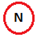
\includegraphics[width=1cm, height=1cm]{./images/N.png} & \textbf{N= ESPECIE NATIVA:} Especie, subespecie o taxón inferior que vive dentro de su área de distribución natural, incluida la zona a la que puede llegar y ocupar utilizando sus sistemas naturales de   dispersión \cite{6}\\
\centering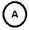
\includegraphics[width=1cm, height=1cm]{./images/a.png} & \textbf{D= Desconocido:} cuando no aparece el taxón ó no aparece  el origen del taxón en la lista patrón de biodiversidad \cite{7}.\\
\centering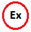
\includegraphics[width=1cm, height=1cm]{./images/EX.png} &\textbf{E= ESPECIE ALÓCTONA (Sinónimo de no-autóctona, exótica):} Especie, subespecie o táxon inferior introducido fuera de su área de distribución natural como resultado de la actividad humana \cite{8, 9}.\\
\hline
\end{tabular}
\end{center}
\caption{}
\label{table3}
\end{table}

\section*{\normalsize{ESTATUS  DEL TAXÓN}}
Incluido como icono, el estatus se organiza en cinco categorías: como especie alóctona,  invasora, criptogénica, criptogénica en expansión o especie en rango de expansión. Junto al icono de estatus se indican las demarcaciones a las que se ha asignado dicho estatus.
El estatus es un concepto dinámico que puede cambiar a medida que se adquiere más información sobre el origen de la especie y/o el vector de introducción. También se tiene en cuenta su extensión en el área introducida y sus efectos e impactos.

\section*{\normalsize{ICONOGRAFÍA}}

\begin{table}[H]
\begin{center}
\begin{tabular}{ >{\centering\arraybackslash}m{2cm} >{\arraybackslash}m{12cm}}
\hline
\rowcolor{green!70!yellow!40}
Simbolo& Definición\\
\hline
\centering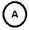
\includegraphics[width=1cm, height=1cm]{./images/a.png} & \textbf{E = ESPECIE ALÓCTONA:} (Sinónimo de no-autóctona, exótica): Especie, subespecie o táxon inferior introducido fuera de su área de distribución natural como resultado de la actividad humana \cite{8,9}, denominándose introducción primaria. A partir de ésta, se puede dar la introducción secundaria, que ocurre sin participación humana, y puede darse por la  propagación por medios naturales, debido a cambios ambientales, como el calentamiento global, o por dispersión por corrientes oceánicas \cite{9, 10}\\
\centering
\includegraphics[width=1cm, height=1cm]{./images/EEI.png} & \textbf{EEI = ESPECIE EXÓTICA INVASORA:} Subconjunto de especies exóticas establecidas, que se han extendido o dispersado en el área de introducción, demostrando su potencial para colonizar otros hábitats y tener efectos adversos sobre la biodiversidad biológica, el funcionamiento de los ecosistemas, la actividad socio-económica o afectar a la salud humana \cite{11,12,13,14}\\
\centering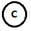
\includegraphics[width=1cm, height=1cm]{./images/C.png} &\textbf{C = ESPECIE CRIPTOGÉNICA:}  Especie que no puede ser clasificada como nativa o como Alóctona, debido a  que no hay evidencias definitivas de su origén exótico, o del modo de introducción desde su área de distribución natural, que puede ser por  tanto una dispersión natural versus a una dispersión mediada por el factor humano (15,16)\\
\centering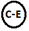
\includegraphics[width=1cm, height=1cm]{./images/CE.png} &\textbf{CRIPTOGÉNICA EN EXPANSIÓN:} Especies con alguna evidencia sobre su condición de Alóctona, pero con incertidumbre debido a un modo de introducción poco claro desde el área de distribución nativa (propagación natural versus mediada por humanos)  \cite{15,16}\\
\centering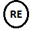
\includegraphics[width=1cm, height=1cm]{./images/RE.png} &\textbf{EXPANSIÓN DE RANGO:} propagación natural de la especie como posible respuesta al cambio climático \cite{15,16}\\
\hline
\end{tabular}
\end{center}
\caption{}
\label{table4}
\end{table}

\section*{\normalsize{NOMBRE ORIGINAL}}
 Muestra en cursiva el nombre científico dado a la especie inicialmente, el autor y el  año de  primera descripción \cite{13,14}.

\section*{NOMBRES COMUNES}
En el caso de existir, éste es incluido.

\section*{NOMBRES EN OTROS IDIOMAS}
Al tratarse de especies alóctonas que no han formado parte de nuestros ecosistemas en muchas ocasiones no existe nombre común, pero puede existir el nombre común en otros idiomas y es incluido.

\section*{SINÓNIMOS}
Con el objetico de facilitar búsquedas de información la especie  puede ser conocida por sinónimos vigentes o no-vigentes, que se han dejado de emplear recientemente, y estos han sido incluidos.

\section*{DESCRIPCIÓN:}
\begin{itemize}
\item Claves de identificación: Apartado para facilitar su identificación. Se incluye una breve descripción de los caracteres más importantes de cada especie. Se trata de una descripción breve, que puede ayudar a la identificación, aunque la identificación correcta de la especie en muchos casos requerirá el uso de una clave taxonómica de identificación y la comprobación de un especialista.  Si existe la posibilidad de que se trate de una especie alóctona se ha de informar sobre su presencia.
\item Imágenes: Se han incluido 1 o 2 imágenes referidas como imagen izquierda (I) e imagen derecha (D). Son fotografías en el medio natural realizadas por diferentes especialistas y observadores del mar, en la mayoría de los casos son fotografías originales (no publicadas).  Se añade un pie de figura de la especie y una breve descripción, incluyendo la autoria de la imagen. 
\item Dificultad de identificación: Al tratarse de especies que presentan similitudes con otras especies, en algunos casos con especies nativas, se ha incluido este apartado que indica el parecido con otras especies, y en una escala de tres niveles la dificultad de identificación a simple vista: BAJA, MEDIA o ALTA.
\end{itemize}


\section*{HABITAT}
En este apartado se describe el hábitat habitual  y el hábitat en que podemos encontrar la especie en la zona de introducida. 

\section*{BIOLOGÍA Y ECOLOGÍA}
Al tratarse de especies alóctonas, para conocer mejor su potencial como invasoras, se ha incluido la descripción de las características de su biología y ecología, con el objetivo de ayudar a conocer mejor las condiciones en que tiene lugar el ciclo vital de la especie. 

\section*{CÓDIGOS DE ACCESO AL GENBANK DE SECUENCIAS DE ADN SELECCIONADAS:} 
Se aportan los códigos genéticos de ADN  cuando existen para cada especie. Se hace con el objetivo de proporcionar información molecular de identificación de la especie, útil si se realizan seguimientos moleculares en EMP, en zonas sensibles, o en puntos de introducción \cite{17, 18}.
Para seleccionar los códigos se han seguido los siguientes criterios: 

\begin{itemize}
\item En algas  macrófitas: las secuencias RBCL o COX1.
\item En fauna invertebrados y vertebrados peces: las secuencias COI, COX1 o 18S. 
\item Siempre que ha sido posible, se han seleccionado secuencias largas de pares de bases de nucleótidos de más 600pb.
\item Preferentemente se han seleccionado secuencias de muestras de zonas próximas. En el caso de que no existan, se han seleccionado las de su área original. 
\item Una vez seleccionados los nucleótidos se ha comprobado que tuviera un porcentaje de identidad del 100\%, para ello se ha utilizado el sistema de búsqueda de alineación local llamado BLAST (Basic Local Alignment Search Tool). Este programa encuentra regiones de similitud local entre secuencias. El programa compara secuencias de nucleótidos o proteínas con bases de datos de secuencias y calcula la significación estadística de las coincidencias. Se puede utilizar para inferir relaciones funcionales y evolutivas entre secuencias, así como para ayudar a identificar grupos de familias de genes. 
\end{itemize}

\section*{DISTRIBUCIÓN ORIGINAL:} 
Con el objetivo de mostrar el origen de la especie se indica para cada una de ellas su procedencia y distribución original. 

\section*{PRIMER REGISTRO EN LA REGIÓN:}
En este apartado se proporciona el año y la localidad del primer registro en la región del Atlántico nordoriental o en el mar Mediterráneo, y se indica el año del primer registro en cada demarcación.  En algunos  caso no se conoce el año exacto, y consta un rango de años como primera introducción, en estos casos se indica el primer año de todos los posibles; en otros casos se da un año aproximado anterior al de la publicación de la primera cita (p. ej. <1996) y en estos casos se indica del mismo modo.

\section*{REGISTROS POSTERIORES Y EVOLUCIÓN}
Con el apoyo del mapa que se proporciona, se muestra  la distribución conocida de la especie en las costas españolas, indicando las diferentes demarcaciones.  El mapa de distribución no debe tomarse como una foto fija incuestionable. Lo que se muestra es la distribución de localizaciones en la que la especie ha sido detectada (puntos), pero no es exhaustiva, solo dada cuenta de todas las geolocalizaciones disponibles de cada especie en las diferentes demarcaciones. Con un triángulo se ha indicado el primer registro para cada subregión. En algunos casos no se indica el  primer registro en el mapa debido a no haber  coordenadas exactas de su localización.

\section*{VÍAS DE INTRODUCCIÓN}
En este apartado se indican los posibles vectores de introducción, que con mayor probabilidad son los que han introducido la especie. Los vectores de introducción que se han tenido en cuenta son los establecidos por el Convenio de Biodiversidad (CBD, 2014) (2) : por el transporte marítimo (polizones) en aguas de lastre o en las comunidades incrustantes (“fouling”) asociadas a estructuras artificiales sumergidas; por escape del confinamiento  en la acuicultura y marisqueo o por suelta intencionada o inentencionada en acuarifilia (escape);  por transporte cotaminante en huéspedes organimos o materiales orgánicos (contaminación) asociados a la acuicultura y el marisqueo y; por dispersión por transporte inentencioanado (secundario) desde pasillos o corredores como el Canal de Suez (corredores). 

\section*{IMPACTOS AMBIENTALES Y SOCIOECONÓMICOS}
Se indican los impactos conocidos, ya sea sobre los hábitats o ecosistemas y especies e impactos socio-económicos o para la salud humana.

\section*{MEDIDAS DE GESTIÓN Y CONTROL} 
Se citas los programas de seguimiento informados a la Dirección General de Costas del MITERD, principalmente para las especies descritas en el catálogo de especies invasoras (R.D. 630/2013). 

\section*{WEBS DE INTERÉS}
Se indican las direcciones de plataformas on-line, webs de interés para consulta, que amplían la información de las fichas.

\section*{REFERENCIAS}
Se incluyen las principales refencias bibliográficas consultadas para cada especie al realizar las fichas

\section*{AUTORÍA DE FICHAS}
Las fichas se han realizado con la  aportación de especialistas participantes en la mesa nacional de expertos. En este apartado se nombra  los co-autores de las fichas.

\section*{AUTORIA DE IMÁGENES}
Las fichas se han realizado con la  aportación fotográfica de especialistas y aficionados a la fotografía submarina. En este apartado se nombra los autores de las imágenes.


\begin{thebibliography}{18}
\bibitem{1}
Streftaris, N., Zenetos, A. 2006. Alien Marine Species in the Mediterranean the 100 “Worst Invasives” and their impacts. Mediterranean Marine Science, 7 (1). 87-118.

\bibitem{2}
CBD, 2014. UNEP/CBD/ SBSTT A/18/9/Add.1. Pathways of introduction of invasive species, their prioritization and management. Montreal, 26 June 2014.  Available online: \url{https://www.cbd.int/doc/meetings/sbstta/sbstta-18/official/sbstta-18-09-add1-en.pdf}(accessed on 8 November 2021)

\bibitem{3}Horton, T.; Kroh, A.; Ahyong, S.; Bailly, N.; Bieler, R.eta. al. (2022). World Register of Marine Species. Available from \url{https://www.marinespecies.org at VLIZ}. Accessed 2022-07-18. doi:10.14284/170

\bibitem{4}Guiry, M.D. \& Guiry, G.M. 2022. AlgaeBase. World-wide electronic publication, National University of Ireland, Galway.

\bibitem{5}FAO 2022. ASFIS List of Species for Fishery Statistics Purposes. Fisheries and Aquaculture Division [online]. Rome. 

\bibitem{6}International Council for the Exploration of the Sea. Code of Practice on the Introduction and Transfer of Marine Organisms (2005).

\bibitem{7}BOE, 2020. Resolución del 18 de diciembre del 2020, por la que se revisa y amplía la lista patrón de las especies silvestres presentes en España.  BOE A-2020-16499

\bibitem{8}UNEP World Conservation Monitoring Centre – Glossary of Biodiversity Terms (\url{http://www.unep-wcmc.org/reception/glossary})

\bibitem{9}DECISIÓN (EU) 2017/848 of 17 Mayo de 2017, por la que se establecen las normas en relación a la lista indicativa de elementos a tener en cuenta en la preparación de las Estrategías Marinas. 

\bibitem{10}BOE, 2013. Real Decreto 630/2013, de 2 de agosto, por el que se regula el Catálogo español de especies Alóctonas Invasoras. BOE-A-2013-8565

\bibitem{11}Zenetos, A., Ovalis, P., Giakoumi, S., Kontadakis, C., Lefkaditou, E., Mpazios, G., Simboura, N., \& Tsiamis, K. (2020a). Saronikos Gulf: a hotspot area for Alien species in the Mediterranean Sea. BioInvasions Records, 9(4): 873-889. DOI: 10.3391/bir.2020.9.

\bibitem{12}Zenetos, A., Çinar, M. E., Pancucci-Papadopoulou, M. A., Harmelin, J. G., Furnari, G., Andaloro, F., Bellou, N., Streftaris, N., \& Zibrowius, H. (2005). Annotated list of marine Alien species in the Mediterranean with records of the worst invasive species. Mediterranean Marine Science, 6(2): 63-118. DOI: 10.12681/mms.186.

\bibitem{13}Zenetos, A., Meriç, E., Verlaque, M., Galli, P., Boudouresque, C. F., Giangrande, A., Cinar, M., \& Bilecenoglu, M. (2008). Additions to the annotated list of marine Alien biota in the Mediterranean with special emphasis on Foraminifera and Parasites. Mediterranean Marine Science, 9(1): 119-166. DOI: 10.12681/mms.146.

\bibitem{14}Tsiamis K, Palialexis A, Stefanova K, Gladan ŽN, Skejić S, Despalatović M, Cvitković I, Dragičević B, Dulčić J, Vidjak O, Bojanić N, Žuljević A, Aplikioti M, Argyrou M, Josephides M, Michailidis N, Jakobsen HH, Staehr PA, Ojaveer H, Lehtiniemi M, Massé C, Zenetos A, Castriota L, Livi S, Mazziotti C, Schembri PJ, Evans J, Bartolo AG, Kabuta SH, Smolders S, Knegtering E, Gittenberger A, Gruszka P, Kraśniewski W, Bartilotti C, Tuaty-Guerra M, Canning-Clode J, Costa AC, Parente MI, Botelho AZ, Micael J, Miodonski JV, Carreira GP, Lopes V, Chainho P, Barberá C, Naddafi R, Florin AB, Barry P, Stebbing PD, Cardoso AC. 2019. Non-indigenous species refined national baseline inventories: A synthesis in the context of the European Union's Marine Strategy Framework Directive. Mar Pollut Bull. 2019 Aug;145:429-435. doi: 10.1016/j.marpolbul.2019.06.012. Epub 2019 Jun 22. PMID: 31590807; PMCID: PMC6689109.

\bibitem{15}Tsiamis K, Palialexis A, Connor D, Antoniadis S, Bartilotti C, Bartolo G.A, Berggreen UC, Boschetti S, Buschbaum C, Canning-Clode J, Carbonell A, Castriota L, Corbeau C, Costa A, Cvitković I, Despalatović M, Dragičević B, Dulčić J, Fortič A, Francé J, Gittenberger A, Gizzi F, Gollasch S, Gruszka P, Hegarty M, Hema T, Jensen K, Josephides M, Kabuta S, Kerckhof F, Kovtun-Kante A, Krakau M, Kraśniewski W, Lackschewitz D, Lehtiniemi M, Lieberum C, Linnamägi M, Lipej L, Livi S, Lundgreen K, Magliozzi C, Massé C, Mavrič B, Michailidis N, Moncheva S, Mozetič P, Naddafi R, Ninčević Gladan Z, Ojaveer H, Olenin S, Orlando-Bonaca M, Ouerghi A, Parente M, Pavlova P, Peterlin M, Pitacco V, Png-Gonzalez L, Rousou M, Sala-Pérez M, Serrano A, Skorupski J, Smolders S, SrebAlóctona e G, Stæhr PA, Stefanova K, Strake S, Tabarcea C, Todorova V, Trkov D, Tuaty-Guerra M, Vidjak O, Zenetos A, Žuljević A, Cardoso AC, 2021. Marine Strategy Framework Directive- Descriptor 2, Non-Indigenous Species, Delivering solid recommendations for setting threshold values for non-indigenous species pressure on European seas, EUR 30640 EN, Publications Office of the European Union, Luxembourg, 2021, ISBN 978-92-76-32257-3, doi:10.2760/035071, JRC124136.

\bibitem{16}Carlton, J.T. (1996). Biological invasions and cryptogenic species. Ecology, 77: 1653-1655.

\bibitem{17}Sayers, E.W., O'Sullivan, C. \& Karsch-Mizrachi, I. (2022). Using GenBank and SRA. Methods in Molecular Biology, 2443: 1-25. doi: 10.1007/978-1-0716-2067-0\_1.  

\bibitem{18}National Library of Medicine. Acceso online: \url{https://blast.ncbi.nlm.nih.gov}
\end{thebibliography}
\clearpage

\section{\textit{Acrothamnion preissii} (Sonder) E.M.Wollaston \cite{acro1}}

{\color{olive}Filo}: Rhodophyta; {\color{olive}Clase}: Florideophyceae; 
{\color{olive}Orden}: Ceramiales; {\color{olive}Familia}: Ceramiaceae; 
{\color{olive}Género}: Acrothamnion; {\color{olive}Especie}: Acrothamnion preissii
\par
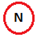
\includegraphics{./images/N.png}

\includegraphics{./images/EEI.png}
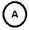
\includegraphics{./images/a.png}
= LEBA		
\par

{\color{olive}Nombre original}: Callithamnion preissii Sonder, 1845
\par 
{\color{olive}Nombres comunes}: no se conocen
\par
{\color{olive}Nombres en otros idiomas}: no se conocen
\section*{MORFOLOGÍA} 
{\color{olive}Claves de identificación}: Talos erectos formados por filamentos uni seriados de color rojo-rosado, de tamaño variable desde 0,5 a 5 cm de alto en el Mediterráneo (imagen izquierda), aunque se ha encontrado talos hasta de 9 cm en el Atlántico (Azores) \cite{acro2,acro5}. Tapizan los fondos formando céspedes de aspecto algodonoso (imagen derecha) \cite{acro2,acro3}. Se puede identificar al microscopio porque las células axiales presentan verticilos de 4 ramas laterales cortas, de las cuales dos son más largas y dos más cortas, se disponen de manera opuesta y, a su vez se ramifican de forma alterna; presentan además células glandulares terminales, característica distintiva de la que sirve para su identificación \cite{acro2,acro5}. En el Mediterráneo, solo se han observado esporófitos, que presentan las tetrásporas en la parte basal de las ramas laterales y orientadas hacia la parte apical de la planta \cite{acro5,acro6}.
\newline
\begin{figure}[h]
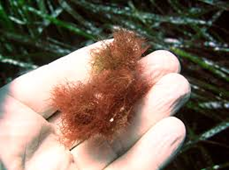
\includegraphics{./images/acro.png}
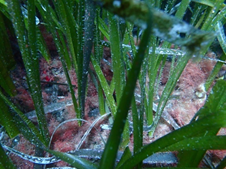
\includegraphics{./images/acro2.png}
\caption{\textit{Acrothamnion preissii} hábito (imagen izquierda) sobre fondo de fanerógamas marinas (imagen derecha)}
\end{figure}

{\color{olive}Dificultad de identificación}: ALTA. Posible confusión con especies que también tapizan el sustrato formando céspedes de aspecto algodonoso. Se puede diferenciar claramente de otras especies similares observando las células glandulares terminales al microscopio.

\section*{HÁBITAT} 
{\color{olive}Hábitat general}: Sobre sustratos rocosos o epífita de macroalgas y fanerógamas marinas, tanto de la zona supramareal como infralitoral.
\par
{\color{olive}Hábitat en la zona introducida}: Crece principalmente de forma epífita sobre rizomas, tanto vivos como muertos, de fanerógamas marinas, principalmente Posidonia, y sobre otras algas. También se ha detectado en el hábitat coralígeno y en fondos de maërl, en zonas de luz atenuada con cierto grado de hidrodinamismo. Se encuentra desde el supramareal hasta 40 m de profundidad \cite{acro3,acro5}.

\section*{BIOLOGÍA Y ECOLOGÍA}
Ciclo trigenético isomórfico en el que alternan las fases de vida libre gametofítica (haploide) y esporofítica (diploide) \cite{acro7}. Especie presente todo el año \cite{acro4}, incluida en el catálogo español de especies invasoras (R.D. 630/2013)\cite{acro8}, considerada entre las 100 especies más invasoras en el Mar Mediterráneo \cite{acro9}. Puede tapizar rizomas de Posidonia y algas de porte erecto, reduciendo la disponibilidad de luz para las especies epifitadas, limitando su desarrollo y comprometiendo su supervivencia.

\section*{CÓDIGOS DE ACCESO AL GENBANK DE SECUENCIAS DE ADN SELECCIONADAS} 
GQ252539 (gen rbcL) \cite{acro10}
\section*{DISTRIBUCIÓN ORIGINAL}
Especie del Indo-Pacífico, nativa de Australia occidental, Japón, Corea y Sudáfrica \cite{acro2}. 
\section*{PRIMER REGISTRO EN LA REGIÓN}
Se registró por primera vez en el Mar Mediterráneo en Italia en 1969, y posteriormente se extendió por la cuenca noroeste, llegando a las Islas Baleares por primera vez en 1993 \cite{acro3,acro5}.
\par
{\color{olive}NOR}
\par
{\color{olive}SUD}
\par
{\color{olive}ESAL}
\par
{\color{olive}LEBA}: 1993 \cite{acro3}
\par
{\color{olive}CAN}
\par

\section*{REGISTROS POSTERIORES Y EVOLUCIÓN}
\begin{figure}[h]
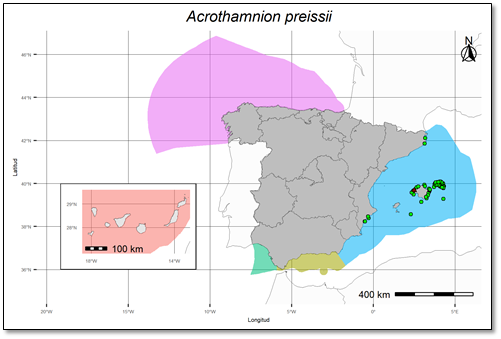
\includegraphics{./images/mapa.png}
\caption{Mapa de geolocalizaciones de \textit{Acrothamnion preissii}}
\end{figure}


\section*{VÍAS DE INTRODUCCIÓN}
Por el transporte marítimo (polizones), en aguas de lastre o en las comunidades incrustantes (“fouling”) asociadas a estructuras artificiales sumergidas, también se ha sugerido su posible introducción por escape de acuarios \cite{acro2}.

\section*{IMPACTOS AMBIENTALES Y SOCIO-ECONÓMICOS}
Desplaza a especies nativas. Se convierte en la epífita dominante sobre las praderas de Posidonia oceanica formando densos céspedes. Provoca pérdidas en la acuicultura, y la pesca comercial y recreativa \cite{acro2}.

\section*{MEDIDAS DE GESTIÓN Y CONTROL}
Programas de seguimientos en Baleares  (IEO\_GOIB), Andalucía (AMAYA), Cataluña (Generalitat de Cataluña Dirección de Medio Ambiente y Biodiversidad).

\section*{WEBS DE INTERÉS}
\url{http://www.marinespecies.org}
\par
\url{https://www.algaebase.org/search/species}
\par
\url{http://www.ciesm.org/atlas/index.html}
\par
\url{http://www.issg.org}
\par
\url{http://www.corpi.ku.lt/databases/index.php/aquanis}
\par
\url{https://www.miteco.gob.es/es/biodiversidad/temas/conservacion-de-especies/especies-exoticas-invasoras/ce-eei-catalogo.aspx}
\par
\url{https://www.ncbi.nlm.nih.gov/genbank/}

\begin{thebibliography}{18}
\bibitem{acro1} Guiry, M.D., \& Guiry, G.M. (2021). AlgaeBase. World-wide electronic publication, National University of Ireland, Galway (taxonomic information republished from AlgaeBase with permission of M.D. Guiry). Acrothamnion preissii (Sonder) E.M.Wollaston, 1968. Accessed through: World Register of Marine Species at: \url{https://www.marinespecies.org/aphia.php?p=taxdetails&id=144488} on 2021-09-09.
\bibitem{acro2}  Verlaque, M., Ruitton, S., Mineur, F., \& Bouderesque, J.-F. (2015). CIESM Atlas of Exotic Species in the Mediterranean, Vol. 4 Macrophytes. CIESM Publishers, Monaco, 362 pp.
\bibitem{acro3} Ferrer, E., Ribera, M.A., \& Gómez Garreta, A. (1994). The spread of Acrothmanion preissii (Sonder) Wollaston (Rhodophyta, Ceramiaceae) in the Mediterranean Sea: new record from the Balearic Islands. Flora Mediterranea, 4: 163-165.
\bibitem{acro4} Klein, J.C., \& Verlaque, M. (2011). Macroalgae newly recorded, rare or introduced to the French Mediterranean coast. Cryptogamie Algologie, 32(2): 111-130.
\bibitem{acro5} Parente, M. I., Gabriel, D., Micael, J., Botelho, A. Z., Ballesteros, E., Milla, D., dos Santos, R., \& Costa, A. C. (2018). First report of the invasive macroalga Acrothamnion preissii (Rhodophyta, Ceramiales) in the Atlantic Ocean. Botanica Marina, 61(1): 85-90. 
\bibitem{acro6} Bottalico, A., Alongi, G., \& Perrone, C. (2016). Macroalgal diversity of Santa Cesarea-Castro (Salento Peninsula, southeastern Italy). Anales del Jardín Botánico de Madrid, 73: 1-12.
\bibitem{acro7} Womersley, H.B.S. (1998). The marine benthic flora of Southern Australia. Rhodophyta. Part IIIC, Ceramiales - Ceramiaceae, Dasyaceae. State Herbarium of South Australia, Adelaide, 535 pp.
\bibitem{acro8} Autor Cooperativo (2013). Fichas del Catálogo Español de Especies Alóctonas Invasoras. RD 630/2013 Ministerio de Agricultura, Alimentación y Medio Ambiente.
\bibitem{acro9} Streftaris, N., \& Zenetos, A. (2006). Alien  Marine Species in the Mediterranean - the 100 ‘Worst Invasives’ and their impact. Mediterranean Marine Science, 7: 87-118. 
\bibitem{acro10} Carlile, A. (2009). Molecular Systematics of North Pacific Ceramiaceae (Rhodophyta): Phylogeny, Taxonomy, and Phylogeography. University of Washington, 296 pp.
\end{thebibliography}

\end{document}
